\documentclass[a4paper,12pt]{article}
\usepackage{HomeWorkTemplate}

\usepackage[utf8]{inputenc}
\usepackage[]{babel}

\setlength{\parindent}{4em}
\setlength{\parskip}{0.5em}

\renewcommand{\baselinestretch}{1.5}

\usepackage{caption}
\usepackage{subcaption}
\usepackage{float}
\usepackage{amsmath}
\usepackage[utf8]{inputenc}
\usepackage{lmodern, textcomp}
\usepackage{circuitikz}
\usepackage[shortlabels]{enumitem}
\usepackage{hyperref}
\usepackage{tikz}
\usepackage{amsmath}
\usepackage{amssymb}
\usepackage{tcolorbox}
\usepackage{graphicx}
\usepackage{xepersian}
\settextfont{XB Niloofar}
\usetikzlibrary{arrows,automata}
\usetikzlibrary{circuits.logic.US}
\usepackage{changepage}
\newcounter{problemcounter}
\newcounter{subproblemcounter}
\setcounter{problemcounter}{1}
\setcounter{subproblemcounter}{1}
\newcommand{\problem}[1]
{
	\subsection*{
		پرسش
		\arabic{problemcounter} 
		\stepcounter{problemcounter}
		\setcounter{subproblemcounter}{1}
		#1
	}
}
\newcommand{\subproblem}{
	\textbf{\harfi{subproblemcounter})}\stepcounter{subproblemcounter}
}


\begin{document}
	\handout
	{اصول پردازش تصویر}
	{دکتر مصطفی کمالی تبریزی}
	{نیم‌سال اول 1399\lr{-}1400}
	{اطلاعیه}
	{سیدعلیرضا خادم}
	{97100398}
	{تمرین سری سوم - سوال پنجم}
	\section*{موارد لازم.}
	برای اجرا لازم است تا تصویر
	\lr{tasbih.jpg}
	در مسیر
	\lr{EX3\_Q5/images/}
	قرار داشته باشد. همچنین در پیاده‌سازی این سوال از کتابخانه‌های 
	\lr{numpy}
	،
	\lr{skimage}
	و
	\lr{cv2}
	استفاده شده است که قبل از اجرا بایستی این کتابخانه‌ها روی سیستم شما نصب باشد.
	\section*{روند کلی حل.}
کلیات روش 
\lr{active contour}‌ای
که پیاده‌سازی شده است مشابه روشی است که در کلاس توضیح داده شده اما یه سری تفاوت‌هایی نیز دارد. که این تفاوت ها عبارت اند از : یکی از تفاوت‌های این پیاده سازی در این است که تعداد راس‌هایی که کانتور را شکل می‌دهند ثابت نیستند و در صورتی که فاصله بین دو راس از یک حدی بیشتر شود یک راس بین این دو راس اضافه می‌شود و همچنین اگر فاصله بین دو راس از حدی کمتر شود یکی از آن رئوس حذف می‌شود.
تفاوت دیگر این پیاده سازی این است که در این پیاده سازی علاوه بر انرژی اینترنال و اکسترنال یک انرژی دیگر تحت عنوان انرژی مرکز اضافه شده است که باعث می‌شود که کانتور بتواند وارد قسمت‌های مقعر شکل نیز بشود. انرژی مرکز به صورت میانگین توان 2 فاصله‌های رئوس از نقاطی که کاربر در ابتدا به عنوان مرکز مشخص می‌کند تعریف ‌می‌شود. (در ابتدای اجرای برنامه که تصویر برای کاربرنمایش داده می‌شود تا منحنی اولیه را مشخص کند، کاربر با کلیک چپ موس می‌تواند رئوس کانتور و با کلیک راست می‌تواند مرکزها را مشخص کند. در صورتی که مرکزی توسط کاربر مشخص نشود، مرکز خود کانتور به عنوان مرکز در نظر گرفته می‌شود، اما توصیه می‌شود با توجه به اینکه آپدیت کردن مرکز کانتور زمان بر است، کاربر خود یک مرکز مانند شکل زیر مشخص کند. البته می‌توانیم متناسب با سوال چند مرکز هم داشته باشیم.)
	\begin{figure}[H]
		\centering
		\begin{subfigure}{0.5\textwidth}
			\centering
			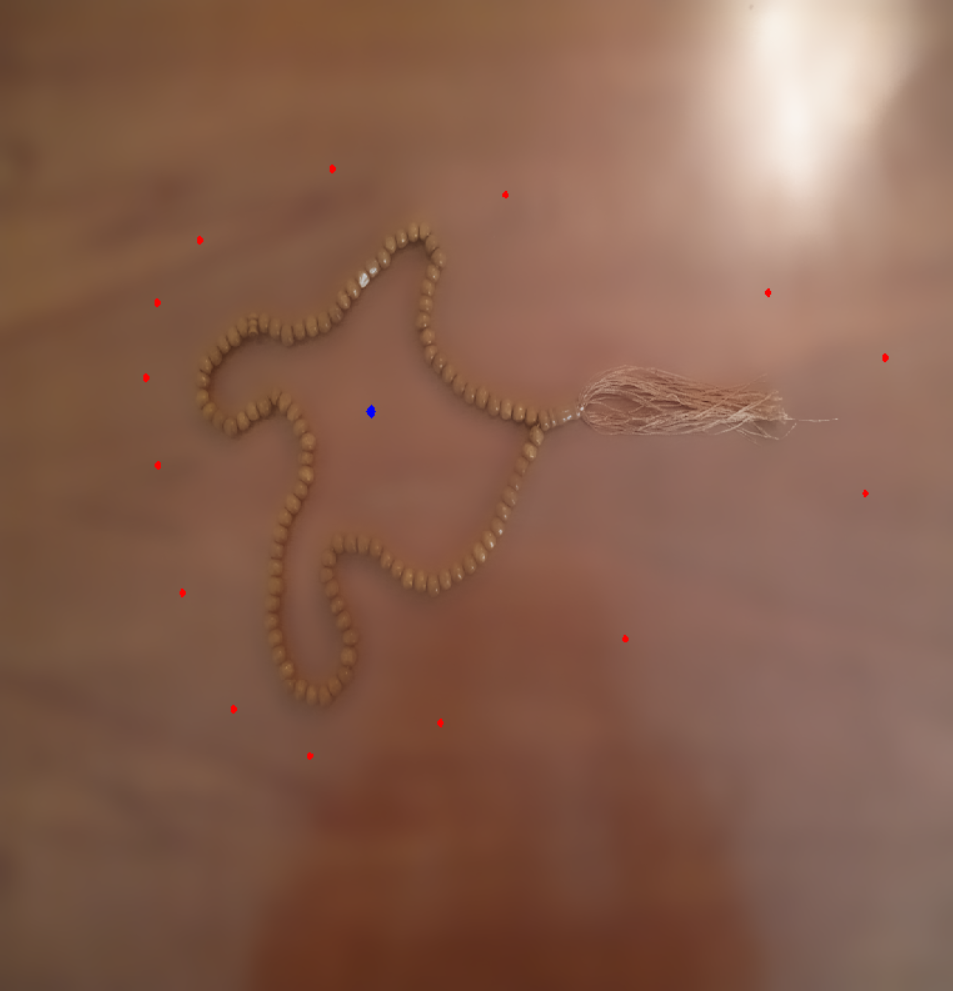
\includegraphics[width=.8\textwidth]{1.png}
		\end{subfigure}
	\end{figure} 
با توجه به اینکه تعداد راس ها متغیر است، متوقف شدن را بر اساس حداکثر تعداد
\lr{iteration}
تعیین می‌کنیم.
	\section*{توضیح کد.}
	برنامه در مجموع حاوی 2 فایل با فرمت
	\lr{.py}
	می‌باشد که توضیحات هر فایل در پایین آمده است.
	\subsection*{$\circ$ utilities.py}
	\subsubsection*{\lr{add\_remove\_vertex(vertices, add\_threshold, remove\_threshold)}}
	این تابع مجموعه راس‌ها را به همراه دو آستانه برای add و remove کردن می‌گیرد و در صورتی که فاصله دو راس از آستانه add بیشتر باشد بین آن‌ها یک راس اضافه می‌کند و اگر فاصله دو راس از آستانه remove کمتر باشد یکی از دو راس را حذف می‌کند.
	\subsubsection*{\lr{cal\_internal\_energy(vertices, index)}}
	این تابع مجموعه رئوس و یک اندیس را به عنوان ورودی می‌گیرد و میزان تاثیر راسی که اندیس به آن اشاره می‌کند و راس بعدی آن را در انرژی درونی محاسبه کرده و به عنوان خروجی برمی‌گرداند.
	\subsubsection*{\lr{cal\_average\_length\_of\_contoure(vertices)}}
	این تابع یک تصویر تابع مجموعه رئوس کانتور را به عنوان ورودی می‌گیرد و میانگین فاصله هر دو راس متوالی را به عنوان خروجی برمی‌گرداند.
	\subsubsection*{\lr{cal\_external\_energy(edge\_detected\_image, vertices, index)}}
	این تابع مجموعه رئوس و یک اندیس و تصویر مرزها را به عنوان ورودی می‌گیرد و میزان تاثیر راسی که اندیس به آن اشاره می‌کند و را در انرژی بیرونی محاسبه کرده و به عنوان خروجی برمی‌گرداند.
	\subsubsection*{\lr{cal\_centers\_energy(vertices, index, centers)}}
	این تابع مجموعه رئوس و یک اندیس و مرکزهارا به عنوان ورودی می‌گیرد و در صورتی که کابر نقطه یا نقاطی را به عنوان مرکز داده باشد مجموع توان 2 فاصله راسی که اندیس به آن اشاره می‌کند، با مرکزها را به عنوان خروجی برمی‌گرداند. در صورتی کاربر هیچ نقطه‌ای را به عنوان مرکز مشخص نکرده باشد توان 2 فاصله راسی که اندیس به آن اشاره می‌کند، با مرکز کانتور را به عنوان خروجی بر‌می‌گرداند.
	\subsubsection*{\lr{cal\_energy(...)}}
	این تابع یه مجموعه راس و تصویر مرز ضرایب انرژی‌ها، میانگین فاصله دو راس مجاور و مرکزها را به عنوان ورودی می‌گیرد و سه انرژی درونی ، بیرونی و مرکز را محاسبه کرده و به عنوان خروجی بر‌می‌گرداند.
	\subsubsection*{\lr{apply\_sobel\_filter\_x(gray\_image)}}
	این تابع یک تصویر سیاه سفید را به عنوان ورودی می‌گیرد و فیلتر sobel\_x را برای پیدا کردن مرزهای عمودی روی تصویر اعمال می‌کند و نتیجه را به توان 2 رسانده و به عنوان خروجی بر‌می‌گرداند.
	\subsubsection*{\lr{apply\_sobel\_filter\_y(gray\_image)}}
	این تابع یک تصویر سیاه سفید را به عنوان ورودی می‌گیرد و فیلتر sobel\_y را برای پیدا کردن مرزهای افقی روی تصویر اعمال می‌کند و نتیجه را به توان 2 رسانده و به عنوان خروجی بر‌می‌گرداند.
	\subsubsection*{\lr{get\_gradient(src\_image)}}
	این تابع یک تصویر را به عنوان ورودی می‌گیرد و بعد از آنکه آن را به تصویر سیاه‌سفید تبدیل با استفاده از توابع \\
	\lr{apply\_sobel\_filter\_x(gray\_image)} و \lr{apply\_sobel\_filter\_y(gray\_image)}
	مرزهای تصویر سیاه‌سفید شده را به دست می‌آورد و به عنوان خروجی بر‌می‌گرداند.
	\subsubsection*{\lr{iteration()}}
	این تابع پیاده سازی active contour با استفاده از برنامه‌نویسی پویا است. تمامی توابعی که در این تابع به کار گرفته شده است توضیح داده شده.\\
	حلقه
	\lr{while}
	تا زمانی که تعداد 
	\lr{iteration}
	ها از 
	\lr{max\_itration}
	کمتر باشد اجرا می‌شود و در هر بار اجرای این حلقه داریم: در ابتدا میانگین توان 2 فاصله بین هر دو راس مجاور با استفاده از تابع 
	\lr{cal\_average\_lenght\_of\_contour}
	محاسبه می‌شود، ماتریس 
	\lr{data}
	با ابعاد 
	$ (k\_window * k\_window, len(vertices), 2) $
	تشکیل می‌دهیم. ماتریس 
	\lr{data}
	همان ماتریسی است که برای حل پیدا کردن بهترین جابه‌جایی در روش برنامه‌ریزی پویا استفاده می‌شود.
	$ data[i, k, 0] $
	نشان‌دهنده این است که اگر راس k از کانتور را در نظر بگیریم و در همسایگی i از آن قرار داشته باشیم بهترین ردیف که می‌توان از ستون k -1 انتخاب کرد تا  از آن به همسایگی i از راس k برسیم و انرژی کمینه بشود. 
	$ data[i, k, 1] $\\
	نشان‌دهنده این است که اگر راس k از کانتور را در نظر بگیریم و در همسایگی i از آن قرار داشته باشیم مجموع انرژی بهترین مسیر تا به اینجا چقدر بوده.\\
	در ادامه جزئیات پیاده‌سازی برنامه‌نویسی پویا آمده است که مطابق با روشی است که در کلاس مطرح شده است.
	\subsubsection*{$\circ$ q5.py} 
	در این فایل ابتدا تصویر 
	\lr{tasbih.jpg}
	را از مسیر
	\lr{EX3\_Q5/images/}
	لود می‌کنیم، بعد یک فیلتر 
	\lr{bilateral}
	روی تصویر اعمال ‌می‌کنیم تا نویزهای تصویر با حفظ مرزها کمتر بشوند. بعد با استفاده از تابع 
	\lr{get\_gradient}
	که تصویر سیاه‌سفید شده را به عنوان ورودی می‌گیرد، مرزهای آن را به‌دست می‌آوریم. در ادامه در  پنجره‌‌ای که برای کاربر نمایش داده می‌شود با کلیک چپ روی تصویر می‌توانیم تعدادی نقطه را برای منحنی اولیه تسبیح انتخاب کنیم. بعد با استفاده از کلیک راست مرکز تسبیح را مانند شکل زیر انتخاب می‌کنیم. بعد از انتخاب کاربر می‌بایست دکمه Esc را بفشارد تا برنامه ادامه پیدا کند.
	\begin{figure}[H]
		\centering
		\begin{subfigure}{0.6\textwidth}
			\centering
			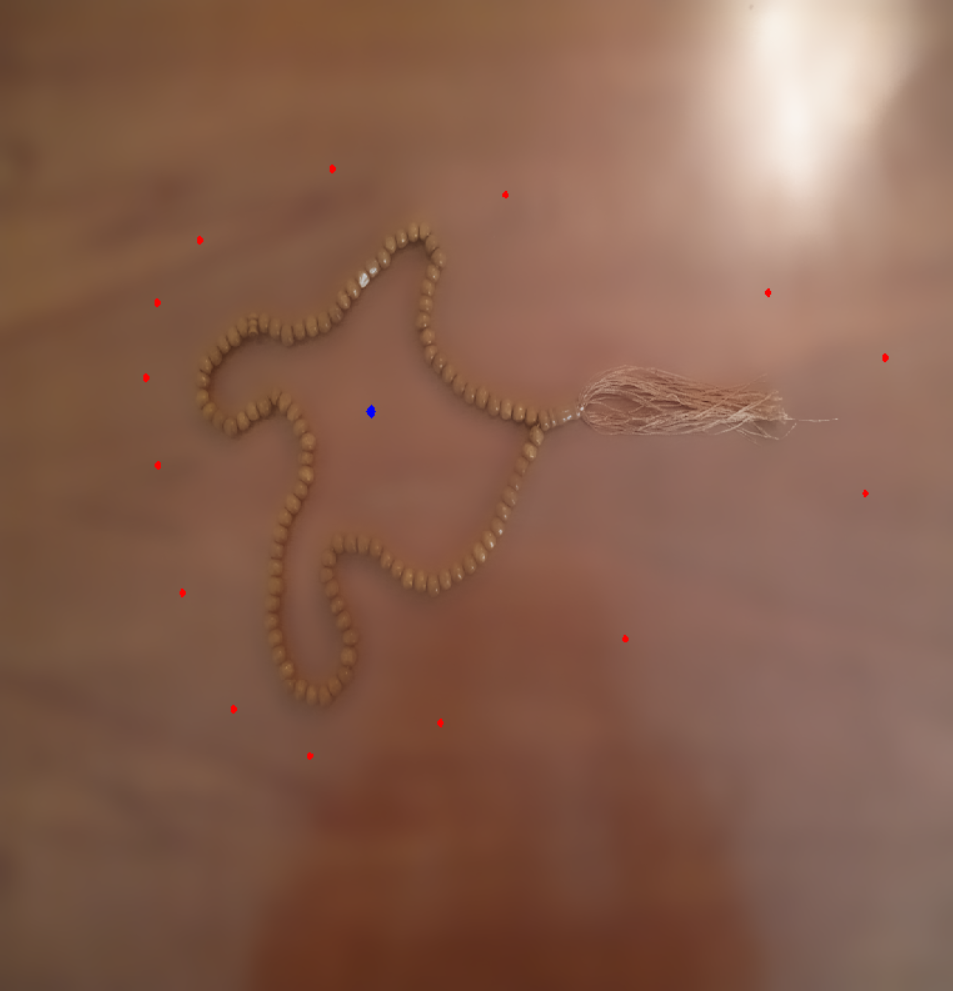
\includegraphics[width=0.8\textwidth]{1.png}
		\end{subfigure}
	\end{figure} 
	در نهایت تابع  
	\lr{iteration}
	 را فراخوانی می‌کنیم تا کانتور حرکت کرده و به مرزهای تسبیح بچشبد.
\end{document}
